
\begin{figure}[H]
\centering
%% Figure 1 (pgfplots). Data: results/paper/zero_readout_n16_8k (seeds 42-51, median and 25th-75th percentile band),
%% results/paper/fig2/n8_s42.json (target A_r) and results/paper/exact_spectra/sigma_sweep/s42_sg0.02.txt (Jacobian J_r).
\definecolor{stepc}{HTML}{0072B2}\definecolor{outc}{HTML}{D55E00}\definecolor{theoc}{HTML}{009E73}
\definecolor{modelc}{HTML}{7B4F9E}\definecolor{mutedc}{HTML}{6E6E6E}
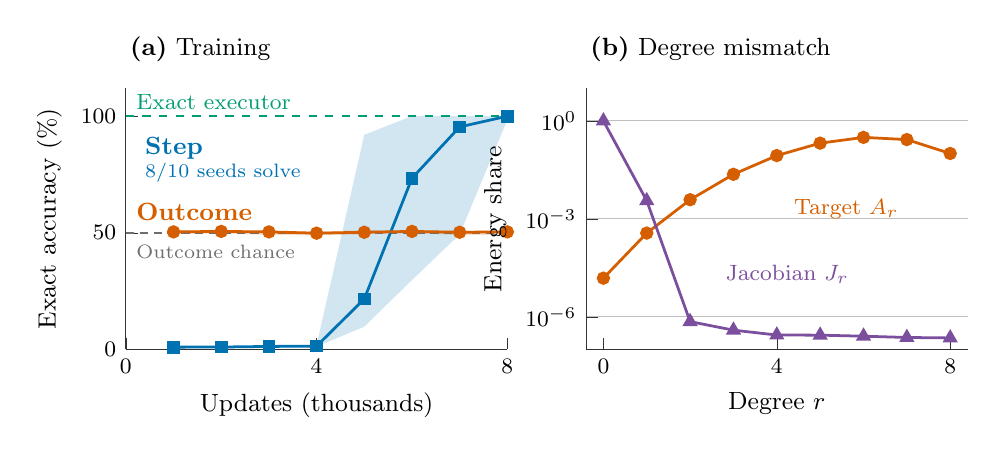
\begin{tikzpicture}
\pgfplotsset{every axis/.style={width=0.53\linewidth, height=4.9cm, axis line style={black!80}, tick style={black!80},
  tick label style={font=\footnotesize}, label style={font=\small}, title style={font=\small, at={(0,1)}, anchor=south west, xshift=-2pt}},
  every axis plot/.append style={line width=1pt}}
\begin{axis}[name=train, title={\textbf{(a)} Training}, xlabel={Updates (thousands)}, ylabel={Exact accuracy (\%)},
  xmin=0, xmax=8, ymin=0, ymax=112, xtick={0,4,8}, ytick={0,50,100}, axis x line*=bottom, axis y line*=left, clip=false]
  \addplot[draw=none, fill=stepc, fill opacity=0.18, forget plot] coordinates {(1,0.55) (2,0.73) (3,0.82) (4,1.25) (5,9.77) (6,29.75) (7,49.33) (8,98.40) (8,100.00) (7,100.00) (6,100.00) (5,92.03) (4,1.90) (3,1.40) (2,1.35) (1,1.35)};
  \addplot[draw=none, fill=outc, fill opacity=0.18, forget plot] coordinates {(1,49.52) (2,49.73) (3,49.05) (4,48.92) (5,49.35) (6,49.92) (7,48.97) (8,49.15) (8,50.70) (7,50.70) (6,51.20) (5,51.08) (4,50.60) (3,50.70) (2,51.08) (1,51.08)};
  \addplot[theoc, dashed, line width=0.9pt, domain=0:8, samples=2] {100};
  \addplot[mutedc, densely dashed, line width=0.8pt, domain=0:8, samples=2] {50};
  \addplot[stepc, mark=square*, mark size=1.8pt] coordinates {(1,1.00) (2,1.05) (3,1.30) (4,1.45) (5,21.65) (6,73.40) (7,95.40) (8,100.00)};
  \addplot[outc, mark=*, mark size=1.9pt] coordinates {(1,50.40) (2,50.60) (3,50.40) (4,49.85) (5,50.25) (6,50.60) (7,50.25) (8,50.40)};
  \node[anchor=south west, font=\footnotesize, text=theoc, inner sep=1pt] at (axis cs:0.15,101.5) {Exact executor};
  \node[anchor=west, font=\small\bfseries, text=stepc] at (axis cs:0.2,86) {Step};
  \node[anchor=west, font=\scriptsize, text=stepc] at (axis cs:0.2,76) {8/10 seeds solve};
  \node[anchor=south west, font=\small\bfseries, text=outc, inner sep=1pt] at (axis cs:0.15,54) {Outcome};
  \node[anchor=north west, font=\scriptsize, text=mutedc, inner sep=1pt] at (axis cs:0.15,46) {Outcome chance};
\end{axis}
\begin{semilogyaxis}[at={(train.east)}, anchor=west, xshift=1.0cm, title={\textbf{(b)} Degree mismatch}, xlabel={Degree $r$},
  ylabel={Energy share}, xmin=-0.4, xmax=8.4, ymin=1e-7, ymax=10, xtick={0,4,8}, ytick={1e-6,1e-3,1},
  ymajorgrids, major grid style={black!25}, axis x line*=bottom, axis y line*=left]
  \addplot[outc, mark=*, mark size=1.9pt] coordinates {(0,1.5259e-05) (1,3.6621e-04) (2,3.8452e-03) (3,2.3071e-02) (4,8.6517e-02) (5,2.0764e-01) (6,3.1146e-01) (7,2.6697e-01) (8,1.0011e-01)};
  \addplot[modelc, mark=triangle*, mark size=2.2pt] coordinates {(0,9.9641e-01) (1,3.5840e-03) (2,7.1281e-07) (3,3.9081e-07) (4,2.7680e-07) (5,2.7450e-07) (6,2.5510e-07) (7,2.3310e-07) (8,2.2560e-07)};
  \node[anchor=north, font=\footnotesize, text=outc] at (axis cs:5.6,8e-3) {Target $A_r$};
  \node[anchor=west, font=\footnotesize, text=modelc] at (axis cs:2.6,2e-5) {Jacobian $J_r$};
\end{semilogyaxis}
\end{tikzpicture}

\caption{\textbf{Training curves and degree mismatch.}
(a)~Counting with $n=16$, $K=2$ and zero readout: median exact continuation accuracy and interquartile band over ten paired seeds, $8$k
updates; the dashed line marks the exact executor that both formats admit (\cref{prop:represent}).
(b)~A separate $n=8$, $K=2$, $\initscale=0.02$ measurement with nonzero readout: target and Jacobian energy occupy different interaction degrees, defined by the number of letters a component depends on jointly (\cref{app:spectrum}).}
\label{fig:overview}
\end{figure}

\begin{figure}[H]
\centering
\resizebox{\linewidth}{!}{%% Figure 4 (pgfplots). Data: results/paper/lambda_grid (20 cells x 3 seeds; cell means with full seed ranges). Spearman rho on cell means.
\definecolor{stepc}{HTML}{0072B2}\definecolor{outc}{HTML}{D55E00}\definecolor{theoc}{HTML}{009E73}
\definecolor{mutedc}{HTML}{6E6E6E}\definecolor{errc}{HTML}{EDB79C}
\begin{tikzpicture}
\pgfplotsset{every axis/.style={width=0.4\linewidth, height=4.9cm, axis line style={black!80}, tick style={black!80},
  tick label style={font=\footnotesize}, label style={font=\small}, title style={font=\small, at={(0,1)}, anchor=south west, xshift=-2pt},
  axis x line*=bottom, axis y line*=left}, every axis plot/.append style={line width=1pt}}
\begin{semilogxaxis}[name=pb, title={\textbf{(a)} Answer bias},
  xlabel={Remaining bias $\mixrate^n$}, ylabel={Outcome accuracy (\%)}, xmin=1e-5, xmax=0.8, xtick={1e-5,1e-3,1e-1},
  ymin=0, ymax=103, ytick={0,50,100}, ymajorgrids, major grid style={black!12}]
  \addplot[mutedc, densely dashed, line width=0.8pt, domain=1e-5:0.8, samples=2] {50};
  \addplot[theoc, dashed, line width=1pt, domain=1e-5:0.7, samples=120] {50*(1+x)};
  \addplot[only marks, outc, mark=*, mark size=1.6pt, error bars/.cd, y dir=both, y explicit, error bar style={errc, line width=0.8pt},
    error mark=none] coordinates {(0.015625,49.6) += (0,0.1) -= (0,0.1) (0.0877915,57.33) += (0,2.467) -= (0,1.633) (0.262144,70.33) += (0,5.667) -= (0,6.233) (0.531441,79.03) += (0,2.167) -= (0,1.933) (0.00390625,51.17) += (0,3.833) -= (0,2.367) (0.0390184,51.27) += (0,1.833) -= (0,2.167) (0.167772,61.73) += (0,3.967) -= (0,3.233) (0.430467,70.93) += (0,0.6667) -= (0,0.5333) (0.000976562,50.07) += (0,0.3333) -= (0,0.5667) (0.0173415,50.57) += (0,0.4333) -= (0,0.8667) (0.107374,55.37) += (0,1.233) -= (0,0.9667) (0.348678,71.13) += (0,2.667) -= (0,2.233) (0.000244141,50.37) += (0,0.5333) -= (0,0.9667) (0.00770735,51.93) += (0,1.467) -= (0,1.433) (0.0687195,51.53) += (0,4.367) -= (0,2.833) (0.28243,64.4) += (0,1.7) -= (0,1.7) (1.52588e-05,50.4) += (0,1.2) -= (0,1.1) (0.00152244,50.2) += (0,1) -= (0,1.3) (0.0281475,50.47) += (0,2.233) -= (0,2.967) (0.185302,57.23) += (0,1.867) -= (0,2.733)};
  \node[anchor=north west, font=\footnotesize] at (rel axis cs:0.03,0.98) {Spearman $\rho=0.91$};
  \node[anchor=north west, font=\footnotesize, text=theoc] at (rel axis cs:0.03,0.8) {State-only prior};
  \node[anchor=north west, font=\scriptsize, text=mutedc] at (rel axis cs:0.03,0.46) {Chance};
\end{semilogxaxis}
\begin{semilogxaxis}[name=pc, at={(pb.east)}, anchor=west, xshift=1.75cm, title={\textbf{(b)} Above the prior},
  xlabel={Remaining bias $\mixrate^n$}, ylabel={Above prior (points)}, xmin=1e-5, xmax=0.8, xtick={1e-5,1e-3,1e-1},
  ymin=-25, ymax=25, ytick={-20,0,20}, ymajorgrids, major grid style={black!12}]
  \addplot[theoc, dashed, line width=1pt, domain=1e-5:0.8, samples=2] {0};
  \addplot[only marks, outc, mark=*, mark size=1.6pt, error bars/.cd, y dir=both, y explicit, error bar style={errc, line width=0.8pt},
    error mark=none] coordinates {(0.015625,-1.181) += (0,0.1) -= (0,0.1) (0.0877915,2.944) += (0,2.467) -= (0,1.633) (0.262144,7.226) += (0,5.667) -= (0,6.233) (0.531441,2.461) += (0,2.167) -= (0,1.933) (0.00390625,0.9714) += (0,3.833) -= (0,2.367) (0.0390184,-0.6843) += (0,1.833) -= (0,2.167) (0.167772,3.345) += (0,3.967) -= (0,3.233) (0.430467,-0.59) += (0,0.6667) -= (0,0.5333) (0.000976562,0.01784) += (0,0.3333) -= (0,0.5667) (0.0173415,-0.3004) += (0,0.4333) -= (0,0.8667) (0.107374,-0.002042) += (0,1.233) -= (0,0.9667) (0.348678,3.699) += (0,2.667) -= (0,2.233) (0.000244141,0.3545) += (0,0.5333) -= (0,0.9667) (0.00770735,1.548) += (0,1.467) -= (0,1.433) (0.0687195,-1.903) += (0,4.367) -= (0,2.833) (0.28243,0.2785) += (0,1.7) -= (0,1.7) (1.52588e-05,0.3992) += (0,1.2) -= (0,1.1) (0.00152244,0.1239) += (0,1) -= (0,1.3) (0.0281475,-0.9407) += (0,2.233) -= (0,2.967) (0.185302,-2.032) += (0,1.867) -= (0,2.733)};
  \node[anchor=north west, font=\footnotesize] at (rel axis cs:0.03,0.98) {Spearman $\rho=0.15$};
  \node[anchor=north west, font=\footnotesize, text=theoc] at (rel axis cs:0.03,0.4) {State-only prior};
\end{semilogxaxis}
\end{tikzpicture}
}
\caption{\textbf{Plateau duration and answer bias.}
(a)~Zero-readout counting, $K=2$, $\mixrate=0.5$, $\initscale=0.002$: median time to a displacement of $0.1\initscale\|\tilde{\bm\theta}\|$ and interquartile band over three draws; the dashed $\mixrate^{-n}$ guide is anchored at $n=4$.
(b)~Outcome exact accuracy after $8$k AdamW updates in $20$ horizon--alphabet cells: means and seed ranges over three seeds; the green curve is the state-only prior $\frac{1+\mixrate^n}{2}$, and gray is chance.
(c)~The same accuracies minus the prior.}
\label{fig:theory-measurement}
\label{fig:lambda-grid}
\end{figure}
